\documentclass[25pt,margin=1in,innermargin=-4.5in,blockverticalspace=-0.25in]{tikzposter}
\geometry{paperwidth=42in,paperheight=32.5in}
\usepackage[utf8]{inputenc}
\usepackage{amsmath}
\usepackage{amsfonts}
\usepackage{amsthm}
\usepackage{amssymb}
\usepackage{mathrsfs}
\usepackage{graphicx}
\usepackage{adjustbox}
\usepackage{enumitem}
\usepackage{UMassTheme}
\usepackage{tikz}
\usetikzlibrary{arrows.meta, decorations.pathmorphing, shapes.geometric}

% set theme parameters
\tikzposterlatexaffectionproofoff
\usetheme{UMassTheme}
\usecolorstyle{UMassStyle}
\usetitlestyle{Filled}

\usepackage[scaled]{helvet}
\renewcommand\familydefault{\sfdefault}
\usepackage[T1]{fontenc}

\title{Borsuk-Ulam Theorem}
\author{Ken Lin}
\institute{Department of Mathematics, University of Massachusetts Amherst}
\titlegraphic{
\includegraphics[width=1.1\textwidth]{UMass Seal Small-Reversed.png}}

\begin{document}
\maketitle
\centering
\begin{columns}

%% ============================================================
%%  COLUMN 1
%% ============================================================
\column{0.32}

\block{Introduction \& Motivation}{
    \begin{quote}
    \itshape
    At any moment, there exist two antipodal points on Earth with \emph{exactly}
    the same temperature and pressure.
    \end{quote}

    \vspace{0.8em}
    This is not a coincidence --- it is a theorem.

    \vspace{0.8em}
    The \textbf{Borsuk-Ulam Theorem} (1933) says that any continuous map from a
    sphere into Euclidean space of one lower dimension must send some pair of
    antipodal points to the same value.

    \vspace{0.8em}
    It was conjectured by Stanislaw Ulam and proved by Karol Borsuk.  The result
    seems geometric but its proof is fundamentally topological --- and its
    consequences reach far beyond geometry.
}

\block{Key Definitions}{
    \begin{itemize}[leftmargin=1.5em, itemsep=0.5em, topsep=0.3em]
        \item $\mathbf{R}$ = real numbers; $\mathbf{C}$ = complex plane;
              $\mathbf{C}^* = \mathbf{C}\setminus\{0\}$ the punctured plane.
        \item \textbf{Sphere:} $S^2 = \{(x,y,z)\in\mathbf{R}^3 : x^2+y^2+z^2=1\}$.
        \item \textbf{Antipodal point:} for $P$ on $S^2$, $P'$ denotes the antipodal point;
              $(x,y,z)' = (-x,-y,-z)$.
        \item \textbf{Closed unit disk:}
              $D = \{z : |z|\leq 1\}$, boundary circle $T = \{z : |z|=1\}$.
        \item $C(X)$: all continuous $f : X \to \mathbf{C}$.
        \item $C^*(X) = \{f\in C(X) : f(X)\subset\mathbf{C}^*\}$: functions that never vanish.
        \item \textbf{Proposition 1:} if $f\in C^*(D)$, there exists $h\in C(D)$ with $e^h = f$.
    \end{itemize}
}

\block{Proof Strategy}{
    Identifying $\mathbf{R}^2$ with $\mathbf{C}$, we regard $F$ as an element
    of $C(S^2)$. The proof proceeds by \textbf{contradiction}.

    \vspace{0.6em}
    \textbf{Step 1 --- Assume no antipodal pair maps equally.}\\
    Suppose $F(P) \neq F(P')$ for all $P$ in $S^2$. Define $G : S^2 \to \mathbf{C}$
    by $G(P) = F(P) - F(P')$. Then $G$ belongs to $C^*(S^2)$, and
    $G(P) = -G(P')$ for all $P$ in $S^2$.

    \vspace{0.6em}
    \textbf{Step 2 --- Parametrize via the upper hemisphere.}\\
    Define $f$ in $C(D)$ by
    \[
        f(x+iy) = G\!\left(x,\,y,\,\sqrt{1-x^2-y^2}\right)
    \]
    (identify the upper hemisphere with the closed unit disk).
    Then $f(z)\neq 0$ for all $z$ in $D$ --- i.e., $f$ belongs to $C^*(D)$ ---
    and $f(z) = -f(-z)$ for all $z$ in $T$.
}

%% ============================================================
%%  COLUMN 2
%% ============================================================
\column{0.36}

\block{}{
    \vspace{0.3em}
    \textbf{Step 3 --- Apply Proposition 1.}\\
    By Proposition 1, there exists $h$ in $C(D)$ such that $f = e^h$.

    \vspace{0.6em}
    \textbf{Step 4 --- Derive the contradiction.}\\
    Let $k(z) = (1/i\pi)[h(z) - h(-z)]$ for $z\in T$.

    \vspace{0.4em}
    For $z\in T$:
    \[
        \exp[i\pi k(z)] = f(z)/f(-z) = -1,
    \]
    so $k(z)$ is an \textbf{odd integer}. Since $k$ is continuous and $T$ is
    connected, $k$ must be constant.

    \vspace{0.4em}
    So we have
    \[
        h(1) = h(-1) + ki\pi = h(1) + 2ki\pi,
    \]
    forcing $k = 0$ --- impossible since $0$ is \textbf{not} an odd integer.
    \textbf{Contradiction.}\quad $\blacksquare$
}

\block{Main Theorem}{
    \textbf{Theorem (Borsuk-Ulam, 1933).}\quad
    \textit{Let $F : S^2 \to \mathbf{R}^2$ be continuous.  Then there exists a
    pair of antipodal points $P$ and $P'$ such that $F(P) = F(P')$.}

    \vspace{0.5em}
    Equivalently: no continuous map $F : S^2 \to \mathbf{R}^2$ can satisfy
    $F(P) \neq F(P')$ for all $P \in S^2$.

    \vspace{0.8em}
    \begin{tikzfigure}[]
    \begin{tikzpicture}[scale=1.0,
        every node/.style={font=\large},
        >=Stealth]
      \draw[line width=2pt] (0,0) circle (2.6cm);
      \draw[line width=1.5pt, dashed] (0,0) ellipse (2.6cm and 0.65cm);
      \fill[UMassMaroon] (0, 2.6) circle (5pt);
      \node[above=4pt] at (0,2.6) {$P$};
      \fill[UMassMaroon] (0,-2.6) circle (5pt);
      \node[below=4pt] at (0,-2.6) {\large$P'$\,(antipodal to $P$)};
      \node[right=6pt] at (2.6,0) {$S^2$};
      \fill[UMassTeal] (7.5,0) circle (6pt);
      \node[right=6pt] at (7.5,0) {$F(P)=F(P')$};
      \node[below=6pt] at (7.5,-0.4) {$\mathbf{R}^2$};
      \draw[->, line width=2pt, UMassTeal]
            (0.15,2.55) .. controls (3,2) .. (7.3,0.12);
      \draw[->, line width=2pt, UMassTeal]
            (0.15,-2.55) .. controls (3,-2) .. (7.3,-0.12);
      \node[above] at (3.5,1.6) {$F$};
    \end{tikzpicture}
    \end{tikzfigure}
}

\block{Application: The Ham Sandwich Theorem}{
    \textbf{Theorem (Stone--Tukey, 1942).}\quad
    \textit{Given any three bounded measurable sets
    $A_1, A_2, A_3 \subset \mathbf{R}^3$, there exists a single plane that
    simultaneously bisects all three.}

    \vspace{0.4em}
    The sets can be in any configuration --- no geometric conditions required.

    \vspace{0.6em}
    \textbf{Proof via Borsuk-Ulam:}

    \vspace{0.4em}
    \textbf{Step 1 (Normal vectors).}\;
    Each point $\mathbf{n} = (n_1, n_2, n_3)$ on the unit sphere $S^2$
    is a unit vector in $\mathbf{R}^3$, i.e.\
    $n_1^2 + n_2^2 + n_3^2 = 1$. We use $\mathbf{n}$ as the
    \emph{normal direction} of a cutting plane.

    \vspace{0.4em}
    \textbf{Step 2 (The bisecting plane $\Pi(\mathbf{n})$).}\;
    For each $\mathbf{n}\in S^2$, consider the family of planes with normal
    $\mathbf{n}$:
    $\{\mathbf{x}\in\mathbf{R}^3 : \mathbf{n}\cdot \mathbf{x} = t\}$, parameterized by $t\in\mathbf{R}$.
    By the intermediate value theorem, there is a unique $t(\mathbf{n})$
    such that this plane bisects $A_1$.  Define
    \[
        \Pi(\mathbf{n})
        \;=\; \bigl\{\mathbf{x}\in\mathbf{R}^3 : \mathbf{n}\cdot \mathbf{x} = t(\mathbf{n})\bigr\}.
    \]
}

%% ============================================================
%%  COLUMN 3
%% ============================================================
\column{0.32}

\block{}{
    \vspace{0.3em}
    \textbf{Step 3 (Signed measure $\mu$).}\;
    Let $\mu$ denote the Lebesgue measure (volume) in $\mathbf{R}^3$.
    The plane $\Pi(\mathbf{n})$ splits each $A_i$ into a positive side
    $A_i^+ = \{\mathbf{x}\in A_i : \mathbf{n}\cdot \mathbf{x} > t(\mathbf{n})\}$ and a
    negative side
    $A_i^- = \{\mathbf{x}\in A_i : \mathbf{n}\cdot \mathbf{x} < t(\mathbf{n})\}$.

    \vspace{0.4em}
    \textbf{Step 4 (The map $F$).}\;
    Define $F : S^2 \to \mathbf{R}^2$ by the volume imbalances of $A_2$
    and $A_3$:
    \[
        F(\mathbf{n})
        \;=\; \bigl(\mu(A_2^+)-\mu(A_2^-),\;\mu(A_3^+)-\mu(A_3^-)\bigr).
    \]
    Note $F$ is continuous.  Flipping $\mathbf{n}\to -\mathbf{n}$ swaps the
    positive and negative sides, so $F(-\mathbf{n}) = -F(\mathbf{n})$.

    \vspace{0.4em}
    \textbf{Step 5 (Apply Borsuk-Ulam).}\;
    By the Borsuk-Ulam theorem, $\exists\,\mathbf{n}^*$ with
    $F(\mathbf{n}^*) = F(-\mathbf{n}^*) = -F(\mathbf{n}^*)$, so
    $F(\mathbf{n}^*) = (0,0)$.

    \vspace{0.4em}
    Thus $\Pi(\mathbf{n}^*)$ bisects $A_2$ and $A_3$ as well, while
    already bisecting $A_1$ by construction.
    \quad$\blacksquare$

    \vspace{0.8em}
    \begin{tikzfigure}[]
        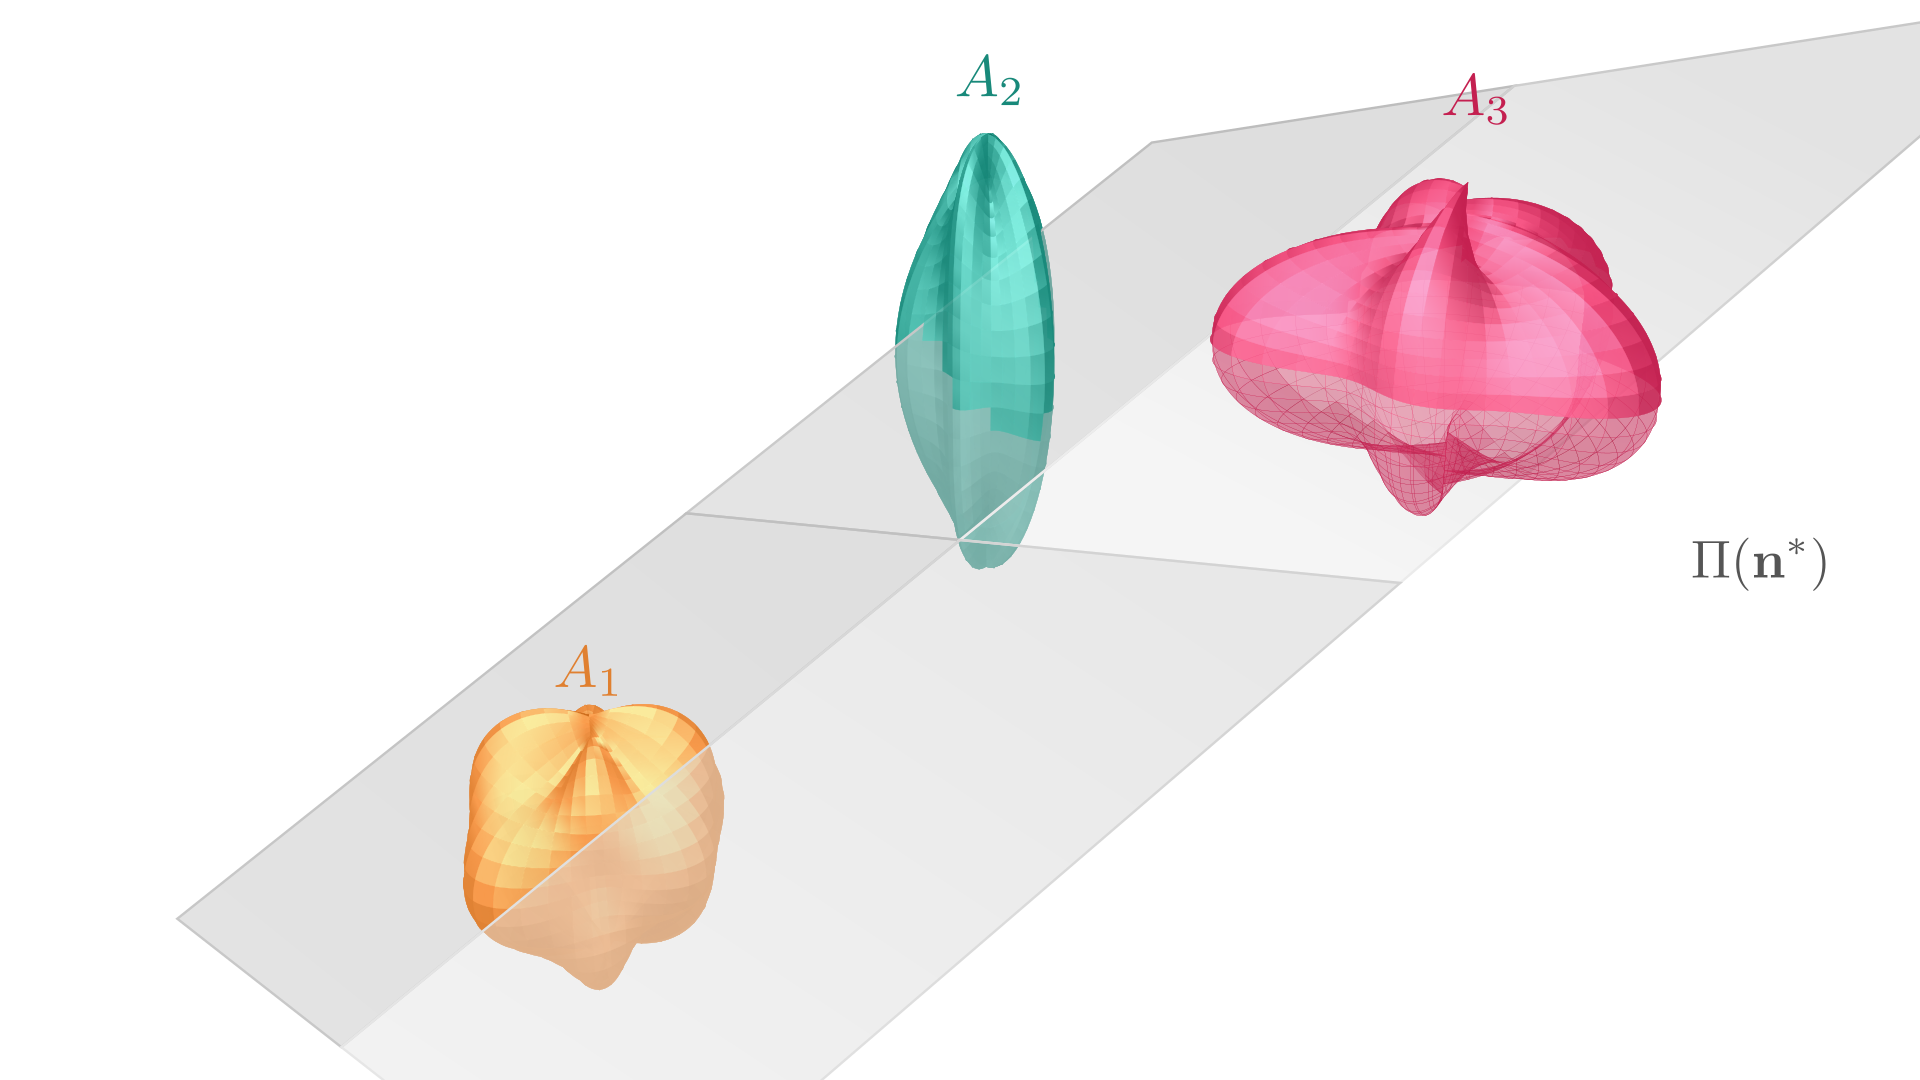
\includegraphics[width=0.78\linewidth]{ham_sandwich.png}
    \end{tikzfigure}
}

\block{Conclusions \& Further Directions}{
    \vspace{0.6em}
    This poster proves the $S^2\to\mathbf{R}^2$ case of the Borsuk-Ulam
    theorem.

    \vspace{0.8em}
    Future work could explore the generalized theorem:
    every continuous map $F:S^n\to\mathbf{R}^n$ identifies some antipodal pair.

    \vspace{0.8em}
    Additionally, one may investigate the generalized Ham Sandwich theorem,
    which states that any $n$ measurable objects in $\mathbf{R}^n$ can be
    simultaneously bisected by a single $(n{-}1)$-dimensional hyperplane.
    \vspace{0.6em}
}

\block{Acknowledgements}{
    {\small
    \begin{itemize}[leftmargin=1.5em, itemsep=0.2em, topsep=0.1em]
        \item UMass Amherst Department of Mathematics, for support and guidance.
        \item 3Blue1Brown, for visual intuition through mathematical animation.
        \item Andrew Browder, for the proof in \textit{Complex Numbers and the
              Ham Sandwich Theorem} (The American Mathematical Monthly, 2006).
    \end{itemize}
    }
}

\end{columns}
\end{document}
